\documentclass[twoside]{article}

% Packages required by doxygen
\usepackage{fixltx2e}
\usepackage{calc}
\usepackage{doxygen}
\usepackage{graphicx}
\usepackage[utf8]{inputenc}
\usepackage{makeidx}
\usepackage{multicol}
\usepackage{multirow}
\PassOptionsToPackage{warn}{textcomp}
\usepackage{textcomp}
\usepackage[nointegrals]{wasysym}
\usepackage[table]{xcolor}

% Font selection
\usepackage[T1]{fontenc}
\usepackage{mathptmx}
\usepackage[scaled=.90]{helvet}
\usepackage{courier}
\usepackage{amssymb}
\usepackage{sectsty}
\renewcommand{\familydefault}{\sfdefault}
\allsectionsfont{%
  \fontseries{bc}\selectfont%
  \color{darkgray}%
}
\renewcommand{\DoxyLabelFont}{%
  \fontseries{bc}\selectfont%
  \color{darkgray}%
}
\newcommand{\+}{\discretionary{\mbox{\scriptsize$\hookleftarrow$}}{}{}}

% Page & text layout
\usepackage{geometry}
\geometry{%
  letterpaper,%
  top=2.5cm,%
  bottom=2.5cm,%
  left=2.5cm,%
  right=2.5cm%
}
\tolerance=750
\hfuzz=15pt
\hbadness=750
\setlength{\emergencystretch}{15pt}
\setlength{\parindent}{0cm}
\setlength{\parskip}{0.2cm}
\makeatletter
\renewcommand{\paragraph}{%
  \@startsection{paragraph}{4}{0ex}{-1.0ex}{1.0ex}{%
    \normalfont\normalsize\bfseries\SS@parafont%
  }%
}
\renewcommand{\subparagraph}{%
  \@startsection{subparagraph}{5}{0ex}{-1.0ex}{1.0ex}{%
    \normalfont\normalsize\bfseries\SS@subparafont%
  }%
}
\makeatother

% Headers & footers
\usepackage{fancyhdr}
\pagestyle{fancyplain}
\fancyhead[LE]{\fancyplain{}{\bfseries\thepage}}
\fancyhead[CE]{\fancyplain{}{}}
\fancyhead[RE]{\fancyplain{}{\bfseries\leftmark}}
\fancyhead[LO]{\fancyplain{}{\bfseries\rightmark}}
\fancyhead[CO]{\fancyplain{}{}}
\fancyhead[RO]{\fancyplain{}{\bfseries\thepage}}
\fancyfoot[LE]{\fancyplain{}{}}
\fancyfoot[CE]{\fancyplain{}{}}
\fancyfoot[RE]{\fancyplain{}{\bfseries\scriptsize Generated on Sat Oct 7 2017 07\+:11\+:12 for C\+S124 Lab3 -\/ Music Program by Doxygen }}
\fancyfoot[LO]{\fancyplain{}{\bfseries\scriptsize Generated on Sat Oct 7 2017 07\+:11\+:12 for C\+S124 Lab3 -\/ Music Program by Doxygen }}
\fancyfoot[CO]{\fancyplain{}{}}
\fancyfoot[RO]{\fancyplain{}{}}
\renewcommand{\footrulewidth}{0.4pt}
\renewcommand{\sectionmark}[1]{%
  \markright{\thesection\ #1}%
}

% Indices & bibliography
\usepackage{natbib}
\usepackage[titles]{tocloft}
\setcounter{tocdepth}{3}
\setcounter{secnumdepth}{5}
\makeindex

% Hyperlinks (required, but should be loaded last)
\usepackage{ifpdf}
\ifpdf
  \usepackage[pdftex,pagebackref=true]{hyperref}
\else
  \usepackage[ps2pdf,pagebackref=true]{hyperref}
\fi
\hypersetup{%
  colorlinks=true,%
  linkcolor=blue,%
  citecolor=blue,%
  unicode%
}

% Custom commands
\newcommand{\clearemptydoublepage}{%
  \newpage{\pagestyle{empty}\cleardoublepage}%
}


%===== C O N T E N T S =====

\begin{document}

% Titlepage & ToC
\hypersetup{pageanchor=false,
             bookmarks=true,
             bookmarksnumbered=true,
             pdfencoding=unicode
            }
\pagenumbering{roman}
\begin{titlepage}
\vspace*{7cm}
\begin{center}%
{\Large C\+S124 Lab3 -\/ Music Program }\\
\vspace*{1cm}
{\large Generated by Doxygen 1.8.8}\\
\vspace*{0.5cm}
{\small Sat Oct 7 2017 07:11:12}\\
\end{center}
\end{titlepage}
\tableofcontents
\pagenumbering{arabic}
\hypersetup{pageanchor=true}

%--- Begin generated contents ---
\section{abc}
\label{abc}
\hypertarget{abc}{}
 
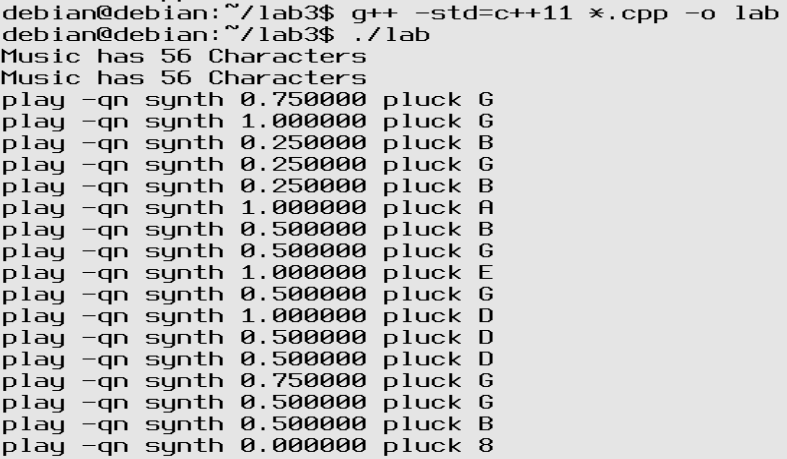
\includegraphics{../lab3.png}



\begin{DoxyVerbInclude}
\end{DoxyVerbInclude}
 
\section{Specification}
\label{Specification}
\hypertarget{Specification}{}
This program has a built in dictionary for english that can be translated to tagalog. It has a user input in which the user may add the translation of a word that is not within the dictionary. 
\section{Analysis}
\label{Analysis}
\hypertarget{Analysis}{}
inputs will be\+:

\begin{DoxyItemize}
\item The outputs will be\+:\end{DoxyItemize}
\begin{DoxyItemize}
\item The overall algorithim is\+: \end{DoxyItemize}

\section{Design}
\label{Design}
\hypertarget{Design}{}
When this program is launched, the user is given the option to choose from any company they would like do their stock exchange. They are given five different companies in a drop down bar to choose from. Once the user has chosen a company, they are given the option to either sell or buy. After the user has chosen one of those two options, the user is then, asked to give their name, shares amount, and price. After the user has entered the following, the program will then execute and insert the information into the heap tree and search through the heap tree. The heap tree will try to find a matching price that the user has input and it will execute the purchase. If there was no match, it will output \char`\"{}\+No seller/buyer\char`\"{} for the user. Also, if the user enter's the name market, it will purchase/sell the shares from the market. After every purchase and sell, it will display in the live graph and live table. The graph and table will update after every transaction. 
\section{Class Index}
\subsection{Class List}
Here are the classes, structs, unions and interfaces with brief descriptions\+:\begin{DoxyCompactList}
\item\contentsline{section}{\hyperlink{structENTRY}{E\+N\+T\+R\+Y} }{\pageref{structENTRY}}{}
\end{DoxyCompactList}

\section{File Index}
\subsection{File List}
Here is a list of all files with brief descriptions\+:\begin{DoxyCompactList}
\item\contentsline{section}{\hyperlink{BuildListDirectly_8cpp}{Build\+List\+Directly.\+cpp} }{\pageref{BuildListDirectly_8cpp}}{}
\item\contentsline{section}{\hyperlink{destroyList_8cpp}{destroy\+List.\+cpp} }{\pageref{destroyList_8cpp}}{}
\item\contentsline{section}{\hyperlink{displayList_8cpp}{display\+List.\+cpp} }{\pageref{displayList_8cpp}}{}
\item\contentsline{section}{\hyperlink{Insert_8cpp}{Insert.\+cpp} }{\pageref{Insert_8cpp}}{}
\item\contentsline{section}{\hyperlink{InsertInOrder_8cpp}{Insert\+In\+Order.\+cpp} }{\pageref{InsertInOrder_8cpp}}{}
\item\contentsline{section}{\hyperlink{lab2_8h}{lab2.\+h} }{\pageref{lab2_8h}}{}
\item\contentsline{section}{\hyperlink{loadList_8cpp}{load\+List.\+cpp} }{\pageref{loadList_8cpp}}{}
\item\contentsline{section}{\hyperlink{loadList2_8cpp}{load\+List2.\+cpp} }{\pageref{loadList2_8cpp}}{}
\item\contentsline{section}{\hyperlink{loadList3_8cpp}{load\+List3.\+cpp} }{\pageref{loadList3_8cpp}}{}
\item\contentsline{section}{\hyperlink{main_8cpp}{main.\+cpp} }{\pageref{main_8cpp}}{}
\end{DoxyCompactList}

\section{Class Documentation}
\hypertarget{structFRAGMENT}{\subsection{F\+R\+A\+G\+M\+E\+N\+T Struct Reference}
\label{structFRAGMENT}\index{F\+R\+A\+G\+M\+E\+N\+T@{F\+R\+A\+G\+M\+E\+N\+T}}
}


{\ttfamily \#include $<$lab3.\+h$>$}

\subsubsection*{Public Attributes}
\begin{DoxyCompactItemize}
\item 
int \hyperlink{structFRAGMENT_a9a2c77dc5f1c259a9a063f8e6ae18724}{start}
\item 
int \hyperlink{structFRAGMENT_a3edee1f345e206cdc220b16d7d290018}{finish}
\end{DoxyCompactItemize}


\subsubsection{Member Data Documentation}
\hypertarget{structFRAGMENT_a3edee1f345e206cdc220b16d7d290018}{\index{F\+R\+A\+G\+M\+E\+N\+T@{F\+R\+A\+G\+M\+E\+N\+T}!finish@{finish}}
\index{finish@{finish}!F\+R\+A\+G\+M\+E\+N\+T@{F\+R\+A\+G\+M\+E\+N\+T}}
\paragraph[{finish}]{\setlength{\rightskip}{0pt plus 5cm}int F\+R\+A\+G\+M\+E\+N\+T\+::finish}}\label{structFRAGMENT_a3edee1f345e206cdc220b16d7d290018}
\hypertarget{structFRAGMENT_a9a2c77dc5f1c259a9a063f8e6ae18724}{\index{F\+R\+A\+G\+M\+E\+N\+T@{F\+R\+A\+G\+M\+E\+N\+T}!start@{start}}
\index{start@{start}!F\+R\+A\+G\+M\+E\+N\+T@{F\+R\+A\+G\+M\+E\+N\+T}}
\paragraph[{start}]{\setlength{\rightskip}{0pt plus 5cm}int F\+R\+A\+G\+M\+E\+N\+T\+::start}}\label{structFRAGMENT_a9a2c77dc5f1c259a9a063f8e6ae18724}


The documentation for this struct was generated from the following file\+:\begin{DoxyCompactItemize}
\item 
\hyperlink{lab3_8h}{lab3.\+h}\end{DoxyCompactItemize}

\hypertarget{structMUSICELMT}{\subsection{M\+U\+S\+I\+C\+E\+L\+M\+T Struct Reference}
\label{structMUSICELMT}\index{M\+U\+S\+I\+C\+E\+L\+M\+T@{M\+U\+S\+I\+C\+E\+L\+M\+T}}
}


{\ttfamily \#include $<$lab3.\+h$>$}



Collaboration diagram for M\+U\+S\+I\+C\+E\+L\+M\+T\+:\nopagebreak
\begin{figure}[H]
\begin{center}
\leavevmode
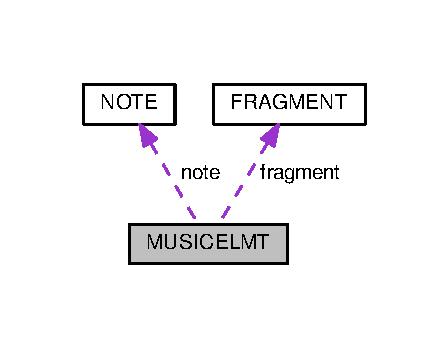
\includegraphics[width=215pt]{structMUSICELMT__coll__graph}
\end{center}
\end{figure}
\subsubsection*{Public Attributes}
\begin{DoxyCompactItemize}
\item 
\hyperlink{lab3_8h_a41c816c739b4ab01c73879f01ae63880}{P\+L\+A\+Y} \hyperlink{structMUSICELMT_aa9a541d279b1a98b190c1968217ad37f}{type}
\item 
\begin{tabbing}
xx\=xx\=xx\=xx\=xx\=xx\=xx\=xx\=xx\=\kill
union \{\\
\>\hyperlink{structNOTE}{NOTE} \hyperlink{structMUSICELMT_a662fdb18330107012ed8902725b08e5c}{note}\\
\>\hyperlink{structFRAGMENT}{FRAGMENT} \hyperlink{structMUSICELMT_ae418bce8087e7510ad8563a87b4c1c63}{fragment}\\
\}; \\

\end{tabbing}\end{DoxyCompactItemize}


\subsubsection{Member Data Documentation}
\hypertarget{structMUSICELMT_af2898ea8d200b7d7c051d968d37e4788}{\paragraph[{"@1}]{\setlength{\rightskip}{0pt plus 5cm}union \{ ... \} }}\label{structMUSICELMT_af2898ea8d200b7d7c051d968d37e4788}
\hypertarget{structMUSICELMT_ae418bce8087e7510ad8563a87b4c1c63}{\index{M\+U\+S\+I\+C\+E\+L\+M\+T@{M\+U\+S\+I\+C\+E\+L\+M\+T}!fragment@{fragment}}
\index{fragment@{fragment}!M\+U\+S\+I\+C\+E\+L\+M\+T@{M\+U\+S\+I\+C\+E\+L\+M\+T}}
\paragraph[{fragment}]{\setlength{\rightskip}{0pt plus 5cm}{\bf F\+R\+A\+G\+M\+E\+N\+T} M\+U\+S\+I\+C\+E\+L\+M\+T\+::fragment}}\label{structMUSICELMT_ae418bce8087e7510ad8563a87b4c1c63}
\hypertarget{structMUSICELMT_a662fdb18330107012ed8902725b08e5c}{\index{M\+U\+S\+I\+C\+E\+L\+M\+T@{M\+U\+S\+I\+C\+E\+L\+M\+T}!note@{note}}
\index{note@{note}!M\+U\+S\+I\+C\+E\+L\+M\+T@{M\+U\+S\+I\+C\+E\+L\+M\+T}}
\paragraph[{note}]{\setlength{\rightskip}{0pt plus 5cm}{\bf N\+O\+T\+E} M\+U\+S\+I\+C\+E\+L\+M\+T\+::note}}\label{structMUSICELMT_a662fdb18330107012ed8902725b08e5c}
\hypertarget{structMUSICELMT_aa9a541d279b1a98b190c1968217ad37f}{\index{M\+U\+S\+I\+C\+E\+L\+M\+T@{M\+U\+S\+I\+C\+E\+L\+M\+T}!type@{type}}
\index{type@{type}!M\+U\+S\+I\+C\+E\+L\+M\+T@{M\+U\+S\+I\+C\+E\+L\+M\+T}}
\paragraph[{type}]{\setlength{\rightskip}{0pt plus 5cm}{\bf P\+L\+A\+Y} M\+U\+S\+I\+C\+E\+L\+M\+T\+::type}}\label{structMUSICELMT_aa9a541d279b1a98b190c1968217ad37f}


The documentation for this struct was generated from the following file\+:\begin{DoxyCompactItemize}
\item 
\hyperlink{lab3_8h}{lab3.\+h}\end{DoxyCompactItemize}

\hypertarget{structNOTE}{\subsection{N\+O\+T\+E Struct Reference}
\label{structNOTE}\index{N\+O\+T\+E@{N\+O\+T\+E}}
}


{\ttfamily \#include $<$lab3.\+h$>$}

\subsubsection*{Public Attributes}
\begin{DoxyCompactItemize}
\item 
char \hyperlink{structNOTE_ae03dbb1306465fe61ec10da05fa5782e}{tone}
\item 
int \hyperlink{structNOTE_a258adf07267f95ab9630b33bad1b2fe2}{duration}
\end{DoxyCompactItemize}


\subsubsection{Member Data Documentation}
\hypertarget{structNOTE_a258adf07267f95ab9630b33bad1b2fe2}{\index{N\+O\+T\+E@{N\+O\+T\+E}!duration@{duration}}
\index{duration@{duration}!N\+O\+T\+E@{N\+O\+T\+E}}
\paragraph[{duration}]{\setlength{\rightskip}{0pt plus 5cm}int N\+O\+T\+E\+::duration}}\label{structNOTE_a258adf07267f95ab9630b33bad1b2fe2}
\hypertarget{structNOTE_ae03dbb1306465fe61ec10da05fa5782e}{\index{N\+O\+T\+E@{N\+O\+T\+E}!tone@{tone}}
\index{tone@{tone}!N\+O\+T\+E@{N\+O\+T\+E}}
\paragraph[{tone}]{\setlength{\rightskip}{0pt plus 5cm}char N\+O\+T\+E\+::tone}}\label{structNOTE_ae03dbb1306465fe61ec10da05fa5782e}


The documentation for this struct was generated from the following file\+:\begin{DoxyCompactItemize}
\item 
\hyperlink{lab3_8h}{lab3.\+h}\end{DoxyCompactItemize}

\hypertarget{structSTACK}{\subsection{S\+T\+A\+C\+K Struct Reference}
\label{structSTACK}\index{S\+T\+A\+C\+K@{S\+T\+A\+C\+K}}
}


{\ttfamily \#include $<$lab3.\+h$>$}

\subsubsection*{Public Attributes}
\begin{DoxyCompactItemize}
\item 
int \hyperlink{structSTACK_ad10f9d8025122e8c82832d7a34c77e40}{size}
\item 
int $\ast$ \hyperlink{structSTACK_a6d512f82cbd75729347a293193039538}{buf}
\item 
int \hyperlink{structSTACK_a1b186cf876dace2f1e30fcbe260cad9a}{sp}
\end{DoxyCompactItemize}


\subsubsection{Member Data Documentation}
\hypertarget{structSTACK_a6d512f82cbd75729347a293193039538}{\index{S\+T\+A\+C\+K@{S\+T\+A\+C\+K}!buf@{buf}}
\index{buf@{buf}!S\+T\+A\+C\+K@{S\+T\+A\+C\+K}}
\paragraph[{buf}]{\setlength{\rightskip}{0pt plus 5cm}int$\ast$ S\+T\+A\+C\+K\+::buf}}\label{structSTACK_a6d512f82cbd75729347a293193039538}
\hypertarget{structSTACK_ad10f9d8025122e8c82832d7a34c77e40}{\index{S\+T\+A\+C\+K@{S\+T\+A\+C\+K}!size@{size}}
\index{size@{size}!S\+T\+A\+C\+K@{S\+T\+A\+C\+K}}
\paragraph[{size}]{\setlength{\rightskip}{0pt plus 5cm}int S\+T\+A\+C\+K\+::size}}\label{structSTACK_ad10f9d8025122e8c82832d7a34c77e40}
\hypertarget{structSTACK_a1b186cf876dace2f1e30fcbe260cad9a}{\index{S\+T\+A\+C\+K@{S\+T\+A\+C\+K}!sp@{sp}}
\index{sp@{sp}!S\+T\+A\+C\+K@{S\+T\+A\+C\+K}}
\paragraph[{sp}]{\setlength{\rightskip}{0pt plus 5cm}int S\+T\+A\+C\+K\+::sp}}\label{structSTACK_a1b186cf876dace2f1e30fcbe260cad9a}


The documentation for this struct was generated from the following file\+:\begin{DoxyCompactItemize}
\item 
\hyperlink{lab3_8h}{lab3.\+h}\end{DoxyCompactItemize}

\section{File Documentation}
\hypertarget{lab_8dox}{\subsection{lab.\+dox File Reference}
\label{lab_8dox}\index{lab.\+dox@{lab.\+dox}}
}

\hypertarget{lab3_8h}{\subsection{lab3.\+h File Reference}
\label{lab3_8h}\index{lab3.\+h@{lab3.\+h}}
}
{\ttfamily \#include $<$iostream$>$}\\*
{\ttfamily \#include $<$string$>$}\\*
{\ttfamily \#include $<$cstdlib$>$}\\*
{\ttfamily \#include $<$fstream$>$}\\*
Include dependency graph for lab3.\+h\+:\nopagebreak
\begin{figure}[H]
\begin{center}
\leavevmode
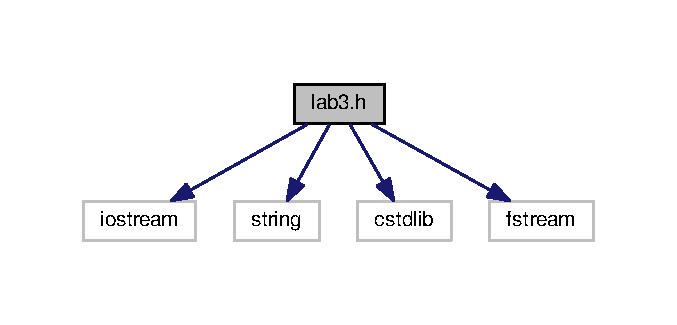
\includegraphics[width=325pt]{lab3_8h__incl}
\end{center}
\end{figure}
This graph shows which files directly or indirectly include this file\+:\nopagebreak
\begin{figure}[H]
\begin{center}
\leavevmode
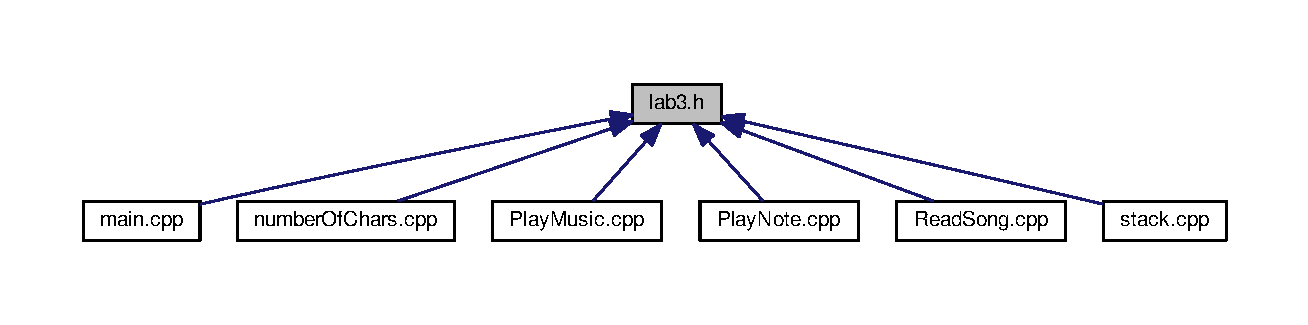
\includegraphics[width=350pt]{lab3_8h__dep__incl}
\end{center}
\end{figure}
\subsubsection*{Classes}
\begin{DoxyCompactItemize}
\item 
struct \hyperlink{structSTACK}{S\+T\+A\+C\+K}
\item 
struct \hyperlink{structNOTE}{N\+O\+T\+E}
\item 
struct \hyperlink{structFRAGMENT}{F\+R\+A\+G\+M\+E\+N\+T}
\item 
struct \hyperlink{structMUSICELMT}{M\+U\+S\+I\+C\+E\+L\+M\+T}
\end{DoxyCompactItemize}
\subsubsection*{Enumerations}
\begin{DoxyCompactItemize}
\item 
enum \hyperlink{lab3_8h_a41c816c739b4ab01c73879f01ae63880}{P\+L\+A\+Y} \{ \hyperlink{lab3_8h_a41c816c739b4ab01c73879f01ae63880a3e1a299c993f58cef9ff1e4853051f02}{P\+L\+A\+Y\+N\+O\+T\+E}, 
\hyperlink{lab3_8h_a41c816c739b4ab01c73879f01ae63880a0fab3b3b81cc5ad4ac6d6b74b50869e5}{P\+L\+A\+Y\+F\+R\+A\+G\+M\+E\+N\+T}, 
\hyperlink{lab3_8h_a41c816c739b4ab01c73879f01ae63880a2175f634cdffa7045d36d1b0cca00ed4}{P\+L\+A\+Y\+S\+T\+O\+P}
 \}
\item 
enum \hyperlink{lab3_8h_a32c27cc471df37f4fc818d65de0a56c4}{S\+T\+A\+T\+U\+S} \{ \hyperlink{lab3_8h_a32c27cc471df37f4fc818d65de0a56c4aecedb56d1405a60c6069f4a0139bdec5}{F\+A\+I\+L\+E\+D}, 
\hyperlink{lab3_8h_a32c27cc471df37f4fc818d65de0a56c4a2bc49ec37d6a5715dd23e85f1ff5bb59}{O\+K}
 \}
\end{DoxyCompactItemize}
\subsubsection*{Functions}
\begin{DoxyCompactItemize}
\item 
\hyperlink{lab3_8h_a32c27cc471df37f4fc818d65de0a56c4}{S\+T\+A\+T\+U\+S} \hyperlink{lab3_8h_abd657d26045a775f57a837427142cfbd}{Create} (\hyperlink{structSTACK}{S\+T\+A\+C\+K} \&stack, int size)
\item 
\hyperlink{lab3_8h_a32c27cc471df37f4fc818d65de0a56c4}{S\+T\+A\+T\+U\+S} \hyperlink{lab3_8h_a805a86f7ac8e643c87ea7d7cbb1b2c9c}{Push} (\hyperlink{structSTACK}{S\+T\+A\+C\+K} \&stack, int item)
\item 
\hyperlink{lab3_8h_a32c27cc471df37f4fc818d65de0a56c4}{S\+T\+A\+T\+U\+S} \hyperlink{lab3_8h_a9ab82590ff3d7086853fd9b2106d255c}{Pop} (\hyperlink{structSTACK}{S\+T\+A\+C\+K} \&stack, int \&item)
\item 
void \hyperlink{lab3_8h_a7f5d0e2c1d5c45b52ee6d1d91e420e95}{Destroy} (\hyperlink{structSTACK}{S\+T\+A\+C\+K} \&stack)
\item 
bool \hyperlink{lab3_8h_a40fe826744e8cbbf7e208d037ef91072}{is\+Empty} (\hyperlink{structSTACK}{S\+T\+A\+C\+K} \&stack)
\item 
bool \hyperlink{lab3_8h_aab5ae433a21f775d4a1874990475da63}{is\+Full} (\hyperlink{structSTACK}{S\+T\+A\+C\+K} \&stack)
\item 
int \hyperlink{lab3_8h_a79338e55dccbfca7203b34ba96644cfd}{No\+Elements} (\hyperlink{structSTACK}{S\+T\+A\+C\+K} \&stack)
\item 
void \hyperlink{lab3_8h_a465df42ae82d3c7db8516dc9d321450e}{read\+Song} (std\+::ifstream \&f, \hyperlink{structMUSICELMT}{M\+U\+S\+I\+C\+E\+L\+M\+T} music\mbox{[}$\,$\mbox{]}, int n)
\item 
void \hyperlink{lab3_8h_a678c8ab56091134ef699893df8a5f683}{Play\+Music} (\hyperlink{structMUSICELMT}{M\+U\+S\+I\+C\+E\+L\+M\+T} music\mbox{[}$\,$\mbox{]}, float tempo)
\item 
void \hyperlink{lab3_8h_ad075a727cdddb38fe5bfa5d055e57161}{Play\+Note} (\hyperlink{structNOTE}{N\+O\+T\+E} \&note, float tempo)
\item 
int \hyperlink{lab3_8h_a1e9336e47067f8c3e92d68bf3a361931}{number\+Of\+Chars} (std\+::ifstream \&f)
\end{DoxyCompactItemize}


\subsubsection{Enumeration Type Documentation}
\hypertarget{lab3_8h_a41c816c739b4ab01c73879f01ae63880}{\index{lab3.\+h@{lab3.\+h}!P\+L\+A\+Y@{P\+L\+A\+Y}}
\index{P\+L\+A\+Y@{P\+L\+A\+Y}!lab3.\+h@{lab3.\+h}}
\paragraph[{P\+L\+A\+Y}]{\setlength{\rightskip}{0pt plus 5cm}enum {\bf P\+L\+A\+Y}}}\label{lab3_8h_a41c816c739b4ab01c73879f01ae63880}
\begin{Desc}
\item[Enumerator]\par
\begin{description}
\index{P\+L\+A\+Y\+N\+O\+T\+E@{P\+L\+A\+Y\+N\+O\+T\+E}!lab3.\+h@{lab3.\+h}}\index{lab3.\+h@{lab3.\+h}!P\+L\+A\+Y\+N\+O\+T\+E@{P\+L\+A\+Y\+N\+O\+T\+E}}\item[{\em 
\hypertarget{lab3_8h_a41c816c739b4ab01c73879f01ae63880a3e1a299c993f58cef9ff1e4853051f02}{P\+L\+A\+Y\+N\+O\+T\+E}\label{lab3_8h_a41c816c739b4ab01c73879f01ae63880a3e1a299c993f58cef9ff1e4853051f02}
}]\index{P\+L\+A\+Y\+F\+R\+A\+G\+M\+E\+N\+T@{P\+L\+A\+Y\+F\+R\+A\+G\+M\+E\+N\+T}!lab3.\+h@{lab3.\+h}}\index{lab3.\+h@{lab3.\+h}!P\+L\+A\+Y\+F\+R\+A\+G\+M\+E\+N\+T@{P\+L\+A\+Y\+F\+R\+A\+G\+M\+E\+N\+T}}\item[{\em 
\hypertarget{lab3_8h_a41c816c739b4ab01c73879f01ae63880a0fab3b3b81cc5ad4ac6d6b74b50869e5}{P\+L\+A\+Y\+F\+R\+A\+G\+M\+E\+N\+T}\label{lab3_8h_a41c816c739b4ab01c73879f01ae63880a0fab3b3b81cc5ad4ac6d6b74b50869e5}
}]\index{P\+L\+A\+Y\+S\+T\+O\+P@{P\+L\+A\+Y\+S\+T\+O\+P}!lab3.\+h@{lab3.\+h}}\index{lab3.\+h@{lab3.\+h}!P\+L\+A\+Y\+S\+T\+O\+P@{P\+L\+A\+Y\+S\+T\+O\+P}}\item[{\em 
\hypertarget{lab3_8h_a41c816c739b4ab01c73879f01ae63880a2175f634cdffa7045d36d1b0cca00ed4}{P\+L\+A\+Y\+S\+T\+O\+P}\label{lab3_8h_a41c816c739b4ab01c73879f01ae63880a2175f634cdffa7045d36d1b0cca00ed4}
}]\end{description}
\end{Desc}

\begin{DoxyCode}
12 \{\hyperlink{lab3_8h_a41c816c739b4ab01c73879f01ae63880a3e1a299c993f58cef9ff1e4853051f02}{PLAYNOTE},\hyperlink{lab3_8h_a41c816c739b4ab01c73879f01ae63880a0fab3b3b81cc5ad4ac6d6b74b50869e5}{PLAYFRAGMENT}, \hyperlink{lab3_8h_a41c816c739b4ab01c73879f01ae63880a2175f634cdffa7045d36d1b0cca00ed4}{PLAYSTOP}\};
\end{DoxyCode}
\hypertarget{lab3_8h_a32c27cc471df37f4fc818d65de0a56c4}{\index{lab3.\+h@{lab3.\+h}!S\+T\+A\+T\+U\+S@{S\+T\+A\+T\+U\+S}}
\index{S\+T\+A\+T\+U\+S@{S\+T\+A\+T\+U\+S}!lab3.\+h@{lab3.\+h}}
\paragraph[{S\+T\+A\+T\+U\+S}]{\setlength{\rightskip}{0pt plus 5cm}enum {\bf S\+T\+A\+T\+U\+S}}}\label{lab3_8h_a32c27cc471df37f4fc818d65de0a56c4}
\begin{Desc}
\item[Enumerator]\par
\begin{description}
\index{F\+A\+I\+L\+E\+D@{F\+A\+I\+L\+E\+D}!lab3.\+h@{lab3.\+h}}\index{lab3.\+h@{lab3.\+h}!F\+A\+I\+L\+E\+D@{F\+A\+I\+L\+E\+D}}\item[{\em 
\hypertarget{lab3_8h_a32c27cc471df37f4fc818d65de0a56c4aecedb56d1405a60c6069f4a0139bdec5}{F\+A\+I\+L\+E\+D}\label{lab3_8h_a32c27cc471df37f4fc818d65de0a56c4aecedb56d1405a60c6069f4a0139bdec5}
}]\index{O\+K@{O\+K}!lab3.\+h@{lab3.\+h}}\index{lab3.\+h@{lab3.\+h}!O\+K@{O\+K}}\item[{\em 
\hypertarget{lab3_8h_a32c27cc471df37f4fc818d65de0a56c4a2bc49ec37d6a5715dd23e85f1ff5bb59}{O\+K}\label{lab3_8h_a32c27cc471df37f4fc818d65de0a56c4a2bc49ec37d6a5715dd23e85f1ff5bb59}
}]\end{description}
\end{Desc}

\begin{DoxyCode}
13 \{\hyperlink{lab3_8h_a32c27cc471df37f4fc818d65de0a56c4aecedb56d1405a60c6069f4a0139bdec5}{FAILED}, \hyperlink{lab3_8h_a32c27cc471df37f4fc818d65de0a56c4a2bc49ec37d6a5715dd23e85f1ff5bb59}{OK}\};
\end{DoxyCode}


\subsubsection{Function Documentation}
\hypertarget{lab3_8h_abd657d26045a775f57a837427142cfbd}{\index{lab3.\+h@{lab3.\+h}!Create@{Create}}
\index{Create@{Create}!lab3.\+h@{lab3.\+h}}
\paragraph[{Create}]{\setlength{\rightskip}{0pt plus 5cm}{\bf S\+T\+A\+T\+U\+S} Create (
\begin{DoxyParamCaption}
\item[{{\bf S\+T\+A\+C\+K} \&}]{stack, }
\item[{int}]{size}
\end{DoxyParamCaption}
)}}\label{lab3_8h_abd657d26045a775f57a837427142cfbd}

\begin{DoxyCode}
10 \{
11     stack.\hyperlink{structSTACK_a6d512f82cbd75729347a293193039538}{buf} = \textcolor{keyword}{new} \textcolor{keywordtype}{int}[size];
12     \textcolor{keywordflow}{if} (!stack.\hyperlink{structSTACK_a6d512f82cbd75729347a293193039538}{buf})
13         \textcolor{keywordflow}{return} \hyperlink{lab3_8h_a32c27cc471df37f4fc818d65de0a56c4aecedb56d1405a60c6069f4a0139bdec5}{FAILED};
14     stack.\hyperlink{structSTACK_ad10f9d8025122e8c82832d7a34c77e40}{size} = size;
15     stack.\hyperlink{structSTACK_a1b186cf876dace2f1e30fcbe260cad9a}{sp} = 0;
16     \textcolor{keywordflow}{return} \hyperlink{lab3_8h_a32c27cc471df37f4fc818d65de0a56c4a2bc49ec37d6a5715dd23e85f1ff5bb59}{OK};
17 \}
\end{DoxyCode}
\hypertarget{lab3_8h_a7f5d0e2c1d5c45b52ee6d1d91e420e95}{\index{lab3.\+h@{lab3.\+h}!Destroy@{Destroy}}
\index{Destroy@{Destroy}!lab3.\+h@{lab3.\+h}}
\paragraph[{Destroy}]{\setlength{\rightskip}{0pt plus 5cm}void Destroy (
\begin{DoxyParamCaption}
\item[{{\bf S\+T\+A\+C\+K} \&}]{stack}
\end{DoxyParamCaption}
)}}\label{lab3_8h_a7f5d0e2c1d5c45b52ee6d1d91e420e95}

\begin{DoxyCode}
44 \{
45     \textcolor{keyword}{delete} [] stack.\hyperlink{structSTACK_a6d512f82cbd75729347a293193039538}{buf};
46 \}
\end{DoxyCode}
\hypertarget{lab3_8h_a40fe826744e8cbbf7e208d037ef91072}{\index{lab3.\+h@{lab3.\+h}!is\+Empty@{is\+Empty}}
\index{is\+Empty@{is\+Empty}!lab3.\+h@{lab3.\+h}}
\paragraph[{is\+Empty}]{\setlength{\rightskip}{0pt plus 5cm}bool is\+Empty (
\begin{DoxyParamCaption}
\item[{{\bf S\+T\+A\+C\+K} \&}]{stack}
\end{DoxyParamCaption}
)\hspace{0.3cm}{\ttfamily [inline]}}}\label{lab3_8h_a40fe826744e8cbbf7e208d037ef91072}

\begin{DoxyCode}
20                                   \{
21         \textcolor{keywordflow}{return} bool(stack.\hyperlink{structSTACK_a1b186cf876dace2f1e30fcbe260cad9a}{sp} ==0);
22 \}
\end{DoxyCode}
\hypertarget{lab3_8h_aab5ae433a21f775d4a1874990475da63}{\index{lab3.\+h@{lab3.\+h}!is\+Full@{is\+Full}}
\index{is\+Full@{is\+Full}!lab3.\+h@{lab3.\+h}}
\paragraph[{is\+Full}]{\setlength{\rightskip}{0pt plus 5cm}bool is\+Full (
\begin{DoxyParamCaption}
\item[{{\bf S\+T\+A\+C\+K} \&}]{stack}
\end{DoxyParamCaption}
)\hspace{0.3cm}{\ttfamily [inline]}}}\label{lab3_8h_aab5ae433a21f775d4a1874990475da63}

\begin{DoxyCode}
24                                  \{
25         \textcolor{keywordflow}{return} bool(stack.\hyperlink{structSTACK_a1b186cf876dace2f1e30fcbe260cad9a}{sp} ==stack.\hyperlink{structSTACK_ad10f9d8025122e8c82832d7a34c77e40}{size});
26 \}
\end{DoxyCode}
\hypertarget{lab3_8h_a79338e55dccbfca7203b34ba96644cfd}{\index{lab3.\+h@{lab3.\+h}!No\+Elements@{No\+Elements}}
\index{No\+Elements@{No\+Elements}!lab3.\+h@{lab3.\+h}}
\paragraph[{No\+Elements}]{\setlength{\rightskip}{0pt plus 5cm}int No\+Elements (
\begin{DoxyParamCaption}
\item[{{\bf S\+T\+A\+C\+K} \&}]{stack}
\end{DoxyParamCaption}
)\hspace{0.3cm}{\ttfamily [inline]}}}\label{lab3_8h_a79338e55dccbfca7203b34ba96644cfd}

\begin{DoxyCode}
28                                     \{
29         \textcolor{keywordflow}{return} stack.\hyperlink{structSTACK_a1b186cf876dace2f1e30fcbe260cad9a}{sp};
30 \}
\end{DoxyCode}
\hypertarget{lab3_8h_a1e9336e47067f8c3e92d68bf3a361931}{\index{lab3.\+h@{lab3.\+h}!number\+Of\+Chars@{number\+Of\+Chars}}
\index{number\+Of\+Chars@{number\+Of\+Chars}!lab3.\+h@{lab3.\+h}}
\paragraph[{number\+Of\+Chars}]{\setlength{\rightskip}{0pt plus 5cm}int number\+Of\+Chars (
\begin{DoxyParamCaption}
\item[{std\+::ifstream \&}]{f}
\end{DoxyParamCaption}
)}}\label{lab3_8h_a1e9336e47067f8c3e92d68bf3a361931}

\begin{DoxyCode}
4 \{
5 
6     \textcolor{keywordtype}{int} n = 0;
7     \textcolor{keywordtype}{char} c;
8     \textcolor{keywordflow}{while}(f >> c)
9         n++;
10     \textcolor{comment}{//count characters}
11     \textcolor{keywordflow}{return} n;
12 
13 \}
\end{DoxyCode}
\hypertarget{lab3_8h_a678c8ab56091134ef699893df8a5f683}{\index{lab3.\+h@{lab3.\+h}!Play\+Music@{Play\+Music}}
\index{Play\+Music@{Play\+Music}!lab3.\+h@{lab3.\+h}}
\paragraph[{Play\+Music}]{\setlength{\rightskip}{0pt plus 5cm}void Play\+Music (
\begin{DoxyParamCaption}
\item[{{\bf M\+U\+S\+I\+C\+E\+L\+M\+T}}]{music\mbox{[}$\,$\mbox{]}, }
\item[{float}]{tempo}
\end{DoxyParamCaption}
)}}\label{lab3_8h_a678c8ab56091134ef699893df8a5f683}

\begin{DoxyCode}
4 \{
5     
6     \textcolor{keyword}{const} \textcolor{keywordtype}{int} MAXSTACK = 400, MAXARRAY = 9999;
7     \hyperlink{structSTACK}{STACK} stack;
8     \hyperlink{lab3_8h_a41c816c739b4ab01c73879f01ae63880}{PLAY} type;
9     
10     \textcolor{keywordflow}{if} (\hyperlink{lab3_8h_abd657d26045a775f57a837427142cfbd}{Create}(stack, MAXSTACK) == \hyperlink{lab3_8h_a32c27cc471df37f4fc818d65de0a56c4aecedb56d1405a60c6069f4a0139bdec5}{FAILED})
11         \{
12             std::cerr << \textcolor{stringliteral}{"*** MUSIC: Stack allocation error. ***\(\backslash\)n"} << std::endl;
13             \textcolor{keywordflow}{return};
14         \}
15     
16     \textcolor{keywordtype}{int} current = 0;
17     \textcolor{keywordtype}{int} finish = MAXARRAY;
18     
19     
20     \textcolor{keywordflow}{while} (\hyperlink{lab3_8h_a32c27cc471df37f4fc818d65de0a56c4a2bc49ec37d6a5715dd23e85f1ff5bb59}{OK}) 
21         \{
22     
23             type = music[current].\hyperlink{structMUSICELMT_aa9a541d279b1a98b190c1968217ad37f}{type};
24             \textcolor{keywordflow}{if} (current <= finish && type != \hyperlink{lab3_8h_a41c816c739b4ab01c73879f01ae63880a2175f634cdffa7045d36d1b0cca00ed4}{PLAYSTOP})
25                 \{
26                     \textcolor{keywordflow}{if} (type == \hyperlink{lab3_8h_a41c816c739b4ab01c73879f01ae63880a3e1a299c993f58cef9ff1e4853051f02}{PLAYNOTE})
27                         \hyperlink{lab3_8h_ad075a727cdddb38fe5bfa5d055e57161}{PlayNote}(music[current++].note, tempo);
28                     \textcolor{keywordflow}{else} \textcolor{keywordflow}{if} (type == \hyperlink{lab3_8h_a41c816c739b4ab01c73879f01ae63880a0fab3b3b81cc5ad4ac6d6b74b50869e5}{PLAYFRAGMENT})
29                         \{
30                             \hyperlink{lab3_8h_a805a86f7ac8e643c87ea7d7cbb1b2c9c}{Push}(stack, current+1);
31                             \hyperlink{lab3_8h_a805a86f7ac8e643c87ea7d7cbb1b2c9c}{Push}(stack, finish);
32                             finish = music[current].\hyperlink{structMUSICELMT_ae418bce8087e7510ad8563a87b4c1c63}{fragment}.\hyperlink{structFRAGMENT_a3edee1f345e206cdc220b16d7d290018}{finish};
33                             current = music[current].\hyperlink{structMUSICELMT_ae418bce8087e7510ad8563a87b4c1c63}{fragment}.\hyperlink{structFRAGMENT_a9a2c77dc5f1c259a9a063f8e6ae18724}{start};
34                         \}
35                 \}
36             \textcolor{keywordflow}{else} \textcolor{keywordflow}{if} (!\hyperlink{lab3_8h_a40fe826744e8cbbf7e208d037ef91072}{isEmpty}(stack))
37                 \{
38                   \hyperlink{lab3_8h_a9ab82590ff3d7086853fd9b2106d255c}{Pop}(stack, finish);
39                   \hyperlink{lab3_8h_a9ab82590ff3d7086853fd9b2106d255c}{Pop}(stack, current);  
40                 \}
41             \textcolor{keywordflow}{else}
42                 \textcolor{comment}{//nothing else to do}
43                 \textcolor{keywordflow}{break};
44     
45         \}
46     \hyperlink{lab3_8h_a7f5d0e2c1d5c45b52ee6d1d91e420e95}{Destroy}(stack);
47 \}
\end{DoxyCode}
\hypertarget{lab3_8h_ad075a727cdddb38fe5bfa5d055e57161}{\index{lab3.\+h@{lab3.\+h}!Play\+Note@{Play\+Note}}
\index{Play\+Note@{Play\+Note}!lab3.\+h@{lab3.\+h}}
\paragraph[{Play\+Note}]{\setlength{\rightskip}{0pt plus 5cm}void Play\+Note (
\begin{DoxyParamCaption}
\item[{{\bf N\+O\+T\+E} \&}]{note, }
\item[{float}]{tempo}
\end{DoxyParamCaption}
)}}\label{lab3_8h_ad075a727cdddb38fe5bfa5d055e57161}

\begin{DoxyCode}
4 \{
5     std::ifstream inputFile(\textcolor{stringliteral}{"music"});
6     \textcolor{keywordtype}{int} n = \hyperlink{lab3_8h_a1e9336e47067f8c3e92d68bf3a361931}{numberOfChars}(inputFile);
7     std::cout << \textcolor{stringliteral}{"Music has "} << n << \textcolor{stringliteral}{" Characters\(\backslash\)n"};
8     inputFile.close();
9     \hyperlink{structMUSICELMT}{MUSICELMT} *music;
10     music = \textcolor{keyword}{new} \hyperlink{structMUSICELMT}{MUSICELMT}[n];
11     inputFile.open(\textcolor{stringliteral}{"music"});
12     \hyperlink{lab3_8h_a465df42ae82d3c7db8516dc9d321450e}{readSong}(inputFile, music, n);
13     inputFile.close();
14         \textcolor{keywordflow}{for}(\textcolor{keywordtype}{int} i=0; i< n; i++)
15         \{
16             \textcolor{keywordflow}{if}(music[i].type == \textcolor{charliteral}{'n'})
17             std::cout << music[i].\hyperlink{structMUSICELMT_a662fdb18330107012ed8902725b08e5c}{note}.\hyperlink{structNOTE_ae03dbb1306465fe61ec10da05fa5782e}{tone} << \textcolor{stringliteral}{" "}
18             << music[i].\hyperlink{structMUSICELMT_a662fdb18330107012ed8902725b08e5c}{note}.\hyperlink{structNOTE_a258adf07267f95ab9630b33bad1b2fe2}{duration} << std::endl;
19         \textcolor{keywordflow}{else} \textcolor{keywordflow}{if}(music[i].type == \textcolor{charliteral}{'f'})
20             std::cout << music[i].\hyperlink{structMUSICELMT_ae418bce8087e7510ad8563a87b4c1c63}{fragment}.\hyperlink{structFRAGMENT_a9a2c77dc5f1c259a9a063f8e6ae18724}{start} << \textcolor{stringliteral}{" "}
21                 << music[i].\hyperlink{structMUSICELMT_ae418bce8087e7510ad8563a87b4c1c63}{fragment}.\hyperlink{structFRAGMENT_a3edee1f345e206cdc220b16d7d290018}{finish} << std::endl;
22         \}
23         std::string s1 = \textcolor{stringliteral}{"play -qn synth "};
24         std::string s2 = \textcolor{stringliteral}{" pluck "};
25         \textcolor{keywordflow}{for} (\textcolor{keywordtype}{int} i = 0; i < n; i++)
26         \{
27         std::string ms = s1 + std:: to\_string(music[i].note.\hyperlink{structNOTE_a258adf07267f95ab9630b33bad1b2fe2}{duration}/16.0)
28                         + s2 + music[i].\hyperlink{structMUSICELMT_a662fdb18330107012ed8902725b08e5c}{note}.\hyperlink{structNOTE_ae03dbb1306465fe61ec10da05fa5782e}{tone};
29         std::cout << ms << std::endl;
30         system(ms.c\_str());
31         
32     \}
33 \}
\end{DoxyCode}
\hypertarget{lab3_8h_a9ab82590ff3d7086853fd9b2106d255c}{\index{lab3.\+h@{lab3.\+h}!Pop@{Pop}}
\index{Pop@{Pop}!lab3.\+h@{lab3.\+h}}
\paragraph[{Pop}]{\setlength{\rightskip}{0pt plus 5cm}{\bf S\+T\+A\+T\+U\+S} Pop (
\begin{DoxyParamCaption}
\item[{{\bf S\+T\+A\+C\+K} \&}]{stack, }
\item[{int \&}]{item}
\end{DoxyParamCaption}
)}}\label{lab3_8h_a9ab82590ff3d7086853fd9b2106d255c}

\begin{DoxyCode}
33 \{
34     
35     \textcolor{keywordflow}{if} (stack.\hyperlink{structSTACK_a1b186cf876dace2f1e30fcbe260cad9a}{sp} == 0)
36         \textcolor{keywordflow}{return} \hyperlink{lab3_8h_a32c27cc471df37f4fc818d65de0a56c4aecedb56d1405a60c6069f4a0139bdec5}{FAILED};
37     stack.\hyperlink{structSTACK_a1b186cf876dace2f1e30fcbe260cad9a}{sp}--;
38     item = stack.\hyperlink{structSTACK_a6d512f82cbd75729347a293193039538}{buf}[stack.\hyperlink{structSTACK_a1b186cf876dace2f1e30fcbe260cad9a}{sp}];
39     \textcolor{keywordflow}{return} \hyperlink{lab3_8h_a32c27cc471df37f4fc818d65de0a56c4a2bc49ec37d6a5715dd23e85f1ff5bb59}{OK};
40 
41 \}
\end{DoxyCode}
\hypertarget{lab3_8h_a805a86f7ac8e643c87ea7d7cbb1b2c9c}{\index{lab3.\+h@{lab3.\+h}!Push@{Push}}
\index{Push@{Push}!lab3.\+h@{lab3.\+h}}
\paragraph[{Push}]{\setlength{\rightskip}{0pt plus 5cm}{\bf S\+T\+A\+T\+U\+S} Push (
\begin{DoxyParamCaption}
\item[{{\bf S\+T\+A\+C\+K} \&}]{stack, }
\item[{int}]{item}
\end{DoxyParamCaption}
)}}\label{lab3_8h_a805a86f7ac8e643c87ea7d7cbb1b2c9c}

\begin{DoxyCode}
23 \{
24 
25     \textcolor{keywordflow}{if} (stack.\hyperlink{structSTACK_a1b186cf876dace2f1e30fcbe260cad9a}{sp} == stack.\hyperlink{structSTACK_ad10f9d8025122e8c82832d7a34c77e40}{size})
26         \textcolor{keywordflow}{return} \hyperlink{lab3_8h_a32c27cc471df37f4fc818d65de0a56c4aecedb56d1405a60c6069f4a0139bdec5}{FAILED};
27     stack.\hyperlink{structSTACK_a6d512f82cbd75729347a293193039538}{buf}[stack.\hyperlink{structSTACK_a1b186cf876dace2f1e30fcbe260cad9a}{sp}] = item;
28     stack.\hyperlink{structSTACK_a1b186cf876dace2f1e30fcbe260cad9a}{sp}++;
29     \textcolor{keywordflow}{return} \hyperlink{lab3_8h_a32c27cc471df37f4fc818d65de0a56c4a2bc49ec37d6a5715dd23e85f1ff5bb59}{OK};
30 \}
\end{DoxyCode}
\hypertarget{lab3_8h_a465df42ae82d3c7db8516dc9d321450e}{\index{lab3.\+h@{lab3.\+h}!read\+Song@{read\+Song}}
\index{read\+Song@{read\+Song}!lab3.\+h@{lab3.\+h}}
\paragraph[{read\+Song}]{\setlength{\rightskip}{0pt plus 5cm}void read\+Song (
\begin{DoxyParamCaption}
\item[{std\+::ifstream \&}]{f, }
\item[{{\bf M\+U\+S\+I\+C\+E\+L\+M\+T}}]{music\mbox{[}$\,$\mbox{]}, }
\item[{int}]{n}
\end{DoxyParamCaption}
)}}\label{lab3_8h_a465df42ae82d3c7db8516dc9d321450e}

\begin{DoxyCode}
5 \{
6     \textcolor{keywordtype}{int} i = 0; \textcolor{keywordtype}{char} type;
7     \textcolor{keywordflow}{while}(f >> type)
8     \{
9         \textcolor{comment}{//type = music[i].type;}
10         \textcolor{keywordflow}{if} (type == \textcolor{charliteral}{'n'})
11             \{
12             f >> music[i].\hyperlink{structMUSICELMT_a662fdb18330107012ed8902725b08e5c}{note}.\hyperlink{structNOTE_ae03dbb1306465fe61ec10da05fa5782e}{tone} >> music[i].\hyperlink{structMUSICELMT_a662fdb18330107012ed8902725b08e5c}{note}.\hyperlink{structNOTE_a258adf07267f95ab9630b33bad1b2fe2}{duration};
13             music[i].\hyperlink{structMUSICELMT_aa9a541d279b1a98b190c1968217ad37f}{type} = \hyperlink{lab3_8h_a41c816c739b4ab01c73879f01ae63880a3e1a299c993f58cef9ff1e4853051f02}{PLAYNOTE};
14             \}
15         \textcolor{keywordflow}{else} \textcolor{keywordflow}{if} (type == \textcolor{charliteral}{'f'})
16             \{
17             f >> music[i].\hyperlink{structMUSICELMT_ae418bce8087e7510ad8563a87b4c1c63}{fragment}.\hyperlink{structFRAGMENT_a9a2c77dc5f1c259a9a063f8e6ae18724}{start} >> music[i].\hyperlink{structMUSICELMT_ae418bce8087e7510ad8563a87b4c1c63}{fragment}.
      \hyperlink{structFRAGMENT_a3edee1f345e206cdc220b16d7d290018}{finish};
18             music[i].\hyperlink{structMUSICELMT_aa9a541d279b1a98b190c1968217ad37f}{type} = \hyperlink{lab3_8h_a41c816c739b4ab01c73879f01ae63880a0fab3b3b81cc5ad4ac6d6b74b50869e5}{PLAYFRAGMENT};
19             \}
20         i++;
21     \}
22     music[i].\hyperlink{structMUSICELMT_aa9a541d279b1a98b190c1968217ad37f}{type} = \hyperlink{lab3_8h_a41c816c739b4ab01c73879f01ae63880a2175f634cdffa7045d36d1b0cca00ed4}{PLAYSTOP};
23 \}
\end{DoxyCode}

\hypertarget{main_8cpp}{\subsection{main.\+cpp File Reference}
\label{main_8cpp}\index{main.\+cpp@{main.\+cpp}}
}
{\ttfamily \#include \char`\"{}lab.\+h\char`\"{}}\\*
Include dependency graph for main.\+cpp\+:\nopagebreak
\begin{figure}[H]
\begin{center}
\leavevmode
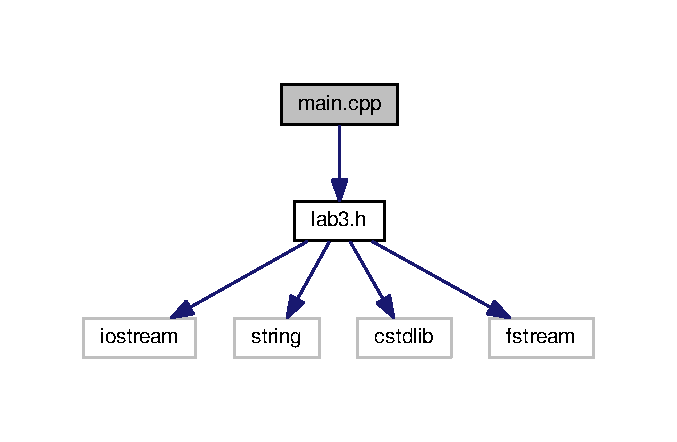
\includegraphics[width=350pt]{main_8cpp__incl}
\end{center}
\end{figure}
\subsubsection*{Functions}
\begin{DoxyCompactItemize}
\item 
int \hyperlink{main_8cpp_ae66f6b31b5ad750f1fe042a706a4e3d4}{main} ()
\end{DoxyCompactItemize}
\subsubsection*{Variables}
\begin{DoxyCompactItemize}
\item 
Fl\+\_\+\+Input $\ast$ \hyperlink{main_8cpp_abf805c82a90897837d1c26ef915f1cd6}{pizza}
\item 
Fl\+\_\+\+Output $\ast$ \hyperlink{main_8cpp_a05c7f6e86cca5f4d0ebf44d1f5042c37}{watch}
\item 
Fl\+\_\+\+Text\+\_\+\+Buffer $\ast$ \hyperlink{main_8cpp_aea2b8efadc87a819fe57c311d668e504}{buff}
\item 
Fl\+\_\+\+Text\+\_\+\+Display $\ast$ \hyperlink{main_8cpp_a23f917547a833922fd6bc8797cc04ee1}{order\+Q}
\end{DoxyCompactItemize}


\subsubsection{Function Documentation}
\hypertarget{main_8cpp_ae66f6b31b5ad750f1fe042a706a4e3d4}{\index{main.\+cpp@{main.\+cpp}!main@{main}}
\index{main@{main}!main.\+cpp@{main.\+cpp}}
\paragraph[{main}]{\setlength{\rightskip}{0pt plus 5cm}int main (
\begin{DoxyParamCaption}
{}
\end{DoxyParamCaption}
)}}\label{main_8cpp_ae66f6b31b5ad750f1fe042a706a4e3d4}

\begin{DoxyCode}
10 \{
11     Fl\_Cairo\_Window cw(400,300); \textcolor{comment}{// width & height of window}
12     cw.label(\textcolor{stringliteral}{"Pizza Deliveries Extravaganja"}); \textcolor{comment}{// title of your cairo window}
13     \textcolor{comment}{//cw.color(FL\_GREEN);}
14     
15     \hyperlink{main_8cpp_abf805c82a90897837d1c26ef915f1cd6}{pizza} = \textcolor{keyword}{new} Fl\_Input(190, 20, 100, 20, \textcolor{stringliteral}{"pizza:"});
16     \hyperlink{main_8cpp_abf805c82a90897837d1c26ef915f1cd6}{pizza}->labelcolor(FL\_BLUE);
17     
18     \hyperlink{main_8cpp_aea2b8efadc87a819fe57c311d668e504}{buff} = \textcolor{keyword}{new} Fl\_Text\_Buffer();
19     \hyperlink{main_8cpp_a23f917547a833922fd6bc8797cc04ee1}{orderQ} = \textcolor{keyword}{new} Fl\_Text\_Display(100,100,100,100,\textcolor{stringliteral}{"Order Q"});
20     \hyperlink{main_8cpp_a23f917547a833922fd6bc8797cc04ee1}{orderQ}->buffer(\hyperlink{main_8cpp_aea2b8efadc87a819fe57c311d668e504}{buff});
21     
22     \hyperlink{main_8cpp_a05c7f6e86cca5f4d0ebf44d1f5042c37}{watch} = \textcolor{keyword}{new} Fl\_Output(70,20,50,20,\textcolor{stringliteral}{"seconds:"});
23     
24     Fl\_Button b(330, 60, 50, 20, \textcolor{stringliteral}{"Order:"});
25     b.callback((Fl\_Callback*)\hyperlink{lab_8h_a547f84331a8c529348e1130ca169c69c}{order\_cb});
26     
27     cw.show();
28     Fl::add\_timeout(1,\hyperlink{lab_8h_a13ed8751dfa95731ad8930762493b16b}{timer});
29     \textcolor{keywordflow}{return} Fl::run();
30 \}
\end{DoxyCode}


\subsubsection{Variable Documentation}
\hypertarget{main_8cpp_aea2b8efadc87a819fe57c311d668e504}{\index{main.\+cpp@{main.\+cpp}!buff@{buff}}
\index{buff@{buff}!main.\+cpp@{main.\+cpp}}
\paragraph[{buff}]{\setlength{\rightskip}{0pt plus 5cm}Fl\+\_\+\+Text\+\_\+\+Buffer$\ast$ buff}}\label{main_8cpp_aea2b8efadc87a819fe57c311d668e504}
\hypertarget{main_8cpp_a23f917547a833922fd6bc8797cc04ee1}{\index{main.\+cpp@{main.\+cpp}!order\+Q@{order\+Q}}
\index{order\+Q@{order\+Q}!main.\+cpp@{main.\+cpp}}
\paragraph[{order\+Q}]{\setlength{\rightskip}{0pt plus 5cm}Fl\+\_\+\+Text\+\_\+\+Display$\ast$ order\+Q}}\label{main_8cpp_a23f917547a833922fd6bc8797cc04ee1}
\hypertarget{main_8cpp_abf805c82a90897837d1c26ef915f1cd6}{\index{main.\+cpp@{main.\+cpp}!pizza@{pizza}}
\index{pizza@{pizza}!main.\+cpp@{main.\+cpp}}
\paragraph[{pizza}]{\setlength{\rightskip}{0pt plus 5cm}Fl\+\_\+\+Input$\ast$ pizza}}\label{main_8cpp_abf805c82a90897837d1c26ef915f1cd6}
\hypertarget{main_8cpp_a05c7f6e86cca5f4d0ebf44d1f5042c37}{\index{main.\+cpp@{main.\+cpp}!watch@{watch}}
\index{watch@{watch}!main.\+cpp@{main.\+cpp}}
\paragraph[{watch}]{\setlength{\rightskip}{0pt plus 5cm}Fl\+\_\+\+Output$\ast$ watch}}\label{main_8cpp_a05c7f6e86cca5f4d0ebf44d1f5042c37}

\hypertarget{numberOfChars_8cpp}{\subsection{number\+Of\+Chars.\+cpp File Reference}
\label{numberOfChars_8cpp}\index{number\+Of\+Chars.\+cpp@{number\+Of\+Chars.\+cpp}}
}
{\ttfamily \#include \char`\"{}lab3.\+h\char`\"{}}\\*
Include dependency graph for number\+Of\+Chars.\+cpp\+:\nopagebreak
\begin{figure}[H]
\begin{center}
\leavevmode
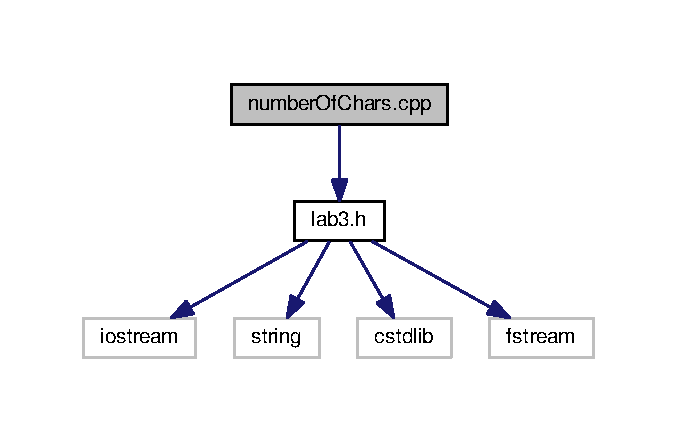
\includegraphics[width=325pt]{numberOfChars_8cpp__incl}
\end{center}
\end{figure}
\subsubsection*{Functions}
\begin{DoxyCompactItemize}
\item 
int \hyperlink{numberOfChars_8cpp_a1e9336e47067f8c3e92d68bf3a361931}{number\+Of\+Chars} (std\+::ifstream \&f)
\end{DoxyCompactItemize}


\subsubsection{Function Documentation}
\hypertarget{numberOfChars_8cpp_a1e9336e47067f8c3e92d68bf3a361931}{\index{number\+Of\+Chars.\+cpp@{number\+Of\+Chars.\+cpp}!number\+Of\+Chars@{number\+Of\+Chars}}
\index{number\+Of\+Chars@{number\+Of\+Chars}!number\+Of\+Chars.\+cpp@{number\+Of\+Chars.\+cpp}}
\paragraph[{number\+Of\+Chars}]{\setlength{\rightskip}{0pt plus 5cm}int number\+Of\+Chars (
\begin{DoxyParamCaption}
\item[{std\+::ifstream \&}]{f}
\end{DoxyParamCaption}
)}}\label{numberOfChars_8cpp_a1e9336e47067f8c3e92d68bf3a361931}

\begin{DoxyCode}
4 \{
5 
6     \textcolor{keywordtype}{int} n = 0;
7     \textcolor{keywordtype}{char} c;
8     \textcolor{keywordflow}{while}(f >> c)
9         n++;
10     \textcolor{comment}{//count characters}
11     \textcolor{keywordflow}{return} n;
12 
13 \}
\end{DoxyCode}

\hypertarget{PlayMusic_8cpp}{\subsection{Play\+Music.\+cpp File Reference}
\label{PlayMusic_8cpp}\index{Play\+Music.\+cpp@{Play\+Music.\+cpp}}
}
{\ttfamily \#include \char`\"{}lab3.\+h\char`\"{}}\\*
Include dependency graph for Play\+Music.\+cpp\+:\nopagebreak
\begin{figure}[H]
\begin{center}
\leavevmode
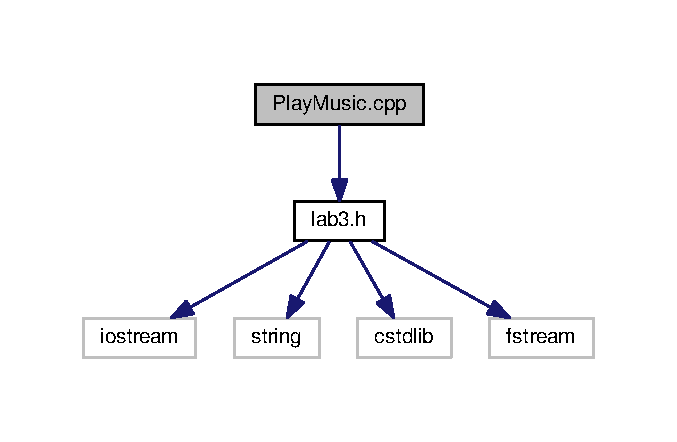
\includegraphics[width=325pt]{PlayMusic_8cpp__incl}
\end{center}
\end{figure}
\subsubsection*{Functions}
\begin{DoxyCompactItemize}
\item 
void \hyperlink{PlayMusic_8cpp_a678c8ab56091134ef699893df8a5f683}{Play\+Music} (\hyperlink{structMUSICELMT}{M\+U\+S\+I\+C\+E\+L\+M\+T} music\mbox{[}$\,$\mbox{]}, float tempo)
\end{DoxyCompactItemize}


\subsubsection{Function Documentation}
\hypertarget{PlayMusic_8cpp_a678c8ab56091134ef699893df8a5f683}{\index{Play\+Music.\+cpp@{Play\+Music.\+cpp}!Play\+Music@{Play\+Music}}
\index{Play\+Music@{Play\+Music}!Play\+Music.\+cpp@{Play\+Music.\+cpp}}
\paragraph[{Play\+Music}]{\setlength{\rightskip}{0pt plus 5cm}void Play\+Music (
\begin{DoxyParamCaption}
\item[{{\bf M\+U\+S\+I\+C\+E\+L\+M\+T}}]{music\mbox{[}$\,$\mbox{]}, }
\item[{float}]{tempo}
\end{DoxyParamCaption}
)}}\label{PlayMusic_8cpp_a678c8ab56091134ef699893df8a5f683}

\begin{DoxyCode}
4 \{
5     
6     \textcolor{keyword}{const} \textcolor{keywordtype}{int} MAXSTACK = 400, MAXARRAY = 9999;
7     \hyperlink{structSTACK}{STACK} stack;
8     \hyperlink{lab3_8h_a41c816c739b4ab01c73879f01ae63880}{PLAY} type;
9     
10     \textcolor{keywordflow}{if} (\hyperlink{lab3_8h_abd657d26045a775f57a837427142cfbd}{Create}(stack, MAXSTACK) == \hyperlink{lab3_8h_a32c27cc471df37f4fc818d65de0a56c4aecedb56d1405a60c6069f4a0139bdec5}{FAILED})
11         \{
12             std::cerr << \textcolor{stringliteral}{"*** MUSIC: Stack allocation error. ***\(\backslash\)n"} << std::endl;
13             \textcolor{keywordflow}{return};
14         \}
15     
16     \textcolor{keywordtype}{int} current = 0;
17     \textcolor{keywordtype}{int} finish = MAXARRAY;
18     
19     
20     \textcolor{keywordflow}{while} (\hyperlink{lab3_8h_a32c27cc471df37f4fc818d65de0a56c4a2bc49ec37d6a5715dd23e85f1ff5bb59}{OK}) 
21         \{
22     
23             type = music[current].\hyperlink{structMUSICELMT_aa9a541d279b1a98b190c1968217ad37f}{type};
24             \textcolor{keywordflow}{if} (current <= finish && type != \hyperlink{lab3_8h_a41c816c739b4ab01c73879f01ae63880a2175f634cdffa7045d36d1b0cca00ed4}{PLAYSTOP})
25                 \{
26                     \textcolor{keywordflow}{if} (type == \hyperlink{lab3_8h_a41c816c739b4ab01c73879f01ae63880a3e1a299c993f58cef9ff1e4853051f02}{PLAYNOTE})
27                         \hyperlink{lab3_8h_ad075a727cdddb38fe5bfa5d055e57161}{PlayNote}(music[current++].note, tempo);
28                     \textcolor{keywordflow}{else} \textcolor{keywordflow}{if} (type == \hyperlink{lab3_8h_a41c816c739b4ab01c73879f01ae63880a0fab3b3b81cc5ad4ac6d6b74b50869e5}{PLAYFRAGMENT})
29                         \{
30                             \hyperlink{lab3_8h_a805a86f7ac8e643c87ea7d7cbb1b2c9c}{Push}(stack, current+1);
31                             \hyperlink{lab3_8h_a805a86f7ac8e643c87ea7d7cbb1b2c9c}{Push}(stack, finish);
32                             finish = music[current].\hyperlink{structMUSICELMT_ae418bce8087e7510ad8563a87b4c1c63}{fragment}.\hyperlink{structFRAGMENT_a3edee1f345e206cdc220b16d7d290018}{finish};
33                             current = music[current].\hyperlink{structMUSICELMT_ae418bce8087e7510ad8563a87b4c1c63}{fragment}.\hyperlink{structFRAGMENT_a9a2c77dc5f1c259a9a063f8e6ae18724}{start};
34                         \}
35                 \}
36             \textcolor{keywordflow}{else} \textcolor{keywordflow}{if} (!\hyperlink{lab3_8h_a40fe826744e8cbbf7e208d037ef91072}{isEmpty}(stack))
37                 \{
38                   \hyperlink{lab3_8h_a9ab82590ff3d7086853fd9b2106d255c}{Pop}(stack, finish);
39                   \hyperlink{lab3_8h_a9ab82590ff3d7086853fd9b2106d255c}{Pop}(stack, current);  
40                 \}
41             \textcolor{keywordflow}{else}
42                 \textcolor{comment}{//nothing else to do}
43                 \textcolor{keywordflow}{break};
44     
45         \}
46     \hyperlink{lab3_8h_a7f5d0e2c1d5c45b52ee6d1d91e420e95}{Destroy}(stack);
47 \}
\end{DoxyCode}

\hypertarget{PlayNote_8cpp}{\subsection{Play\+Note.\+cpp File Reference}
\label{PlayNote_8cpp}\index{Play\+Note.\+cpp@{Play\+Note.\+cpp}}
}
{\ttfamily \#include \char`\"{}lab3.\+h\char`\"{}}\\*
Include dependency graph for Play\+Note.\+cpp\+:\nopagebreak
\begin{figure}[H]
\begin{center}
\leavevmode
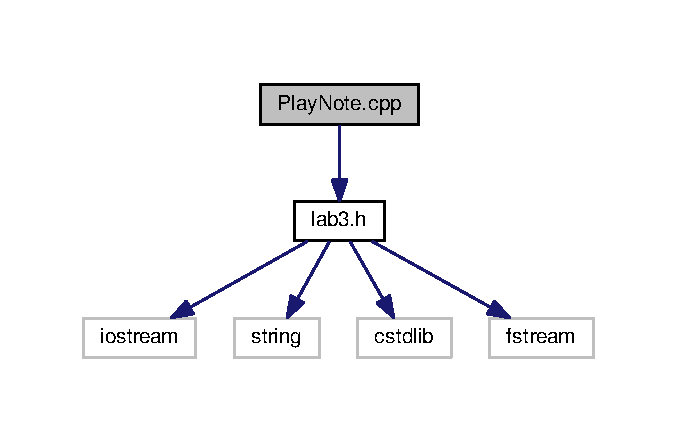
\includegraphics[width=325pt]{PlayNote_8cpp__incl}
\end{center}
\end{figure}
\subsubsection*{Functions}
\begin{DoxyCompactItemize}
\item 
void \hyperlink{PlayNote_8cpp_ad075a727cdddb38fe5bfa5d055e57161}{Play\+Note} (\hyperlink{structNOTE}{N\+O\+T\+E} \&note, float tempo)
\end{DoxyCompactItemize}


\subsubsection{Function Documentation}
\hypertarget{PlayNote_8cpp_ad075a727cdddb38fe5bfa5d055e57161}{\index{Play\+Note.\+cpp@{Play\+Note.\+cpp}!Play\+Note@{Play\+Note}}
\index{Play\+Note@{Play\+Note}!Play\+Note.\+cpp@{Play\+Note.\+cpp}}
\paragraph[{Play\+Note}]{\setlength{\rightskip}{0pt plus 5cm}void Play\+Note (
\begin{DoxyParamCaption}
\item[{{\bf N\+O\+T\+E} \&}]{note, }
\item[{float}]{tempo}
\end{DoxyParamCaption}
)}}\label{PlayNote_8cpp_ad075a727cdddb38fe5bfa5d055e57161}

\begin{DoxyCode}
4 \{
5     std::ifstream inputFile(\textcolor{stringliteral}{"music"});
6     \textcolor{keywordtype}{int} n = \hyperlink{lab3_8h_a1e9336e47067f8c3e92d68bf3a361931}{numberOfChars}(inputFile);
7     std::cout << \textcolor{stringliteral}{"Music has "} << n << \textcolor{stringliteral}{" Characters\(\backslash\)n"};
8     inputFile.close();
9     \hyperlink{structMUSICELMT}{MUSICELMT} *music;
10     music = \textcolor{keyword}{new} \hyperlink{structMUSICELMT}{MUSICELMT}[n];
11     inputFile.open(\textcolor{stringliteral}{"music"});
12     \hyperlink{lab3_8h_a465df42ae82d3c7db8516dc9d321450e}{readSong}(inputFile, music, n);
13     inputFile.close();
14         \textcolor{keywordflow}{for}(\textcolor{keywordtype}{int} i=0; i< n; i++)
15         \{
16             \textcolor{keywordflow}{if}(music[i].type == \textcolor{charliteral}{'n'})
17             std::cout << music[i].\hyperlink{structMUSICELMT_a662fdb18330107012ed8902725b08e5c}{note}.\hyperlink{structNOTE_ae03dbb1306465fe61ec10da05fa5782e}{tone} << \textcolor{stringliteral}{" "}
18             << music[i].\hyperlink{structMUSICELMT_a662fdb18330107012ed8902725b08e5c}{note}.\hyperlink{structNOTE_a258adf07267f95ab9630b33bad1b2fe2}{duration} << std::endl;
19         \textcolor{keywordflow}{else} \textcolor{keywordflow}{if}(music[i].type == \textcolor{charliteral}{'f'})
20             std::cout << music[i].\hyperlink{structMUSICELMT_ae418bce8087e7510ad8563a87b4c1c63}{fragment}.\hyperlink{structFRAGMENT_a9a2c77dc5f1c259a9a063f8e6ae18724}{start} << \textcolor{stringliteral}{" "}
21                 << music[i].\hyperlink{structMUSICELMT_ae418bce8087e7510ad8563a87b4c1c63}{fragment}.\hyperlink{structFRAGMENT_a3edee1f345e206cdc220b16d7d290018}{finish} << std::endl;
22         \}
23         std::string s1 = \textcolor{stringliteral}{"play -qn synth "};
24         std::string s2 = \textcolor{stringliteral}{" pluck "};
25         \textcolor{keywordflow}{for} (\textcolor{keywordtype}{int} i = 0; i < n; i++)
26         \{
27         std::string ms = s1 + std:: to\_string(music[i].note.\hyperlink{structNOTE_a258adf07267f95ab9630b33bad1b2fe2}{duration}/16.0)
28                         + s2 + music[i].\hyperlink{structMUSICELMT_a662fdb18330107012ed8902725b08e5c}{note}.\hyperlink{structNOTE_ae03dbb1306465fe61ec10da05fa5782e}{tone};
29         std::cout << ms << std::endl;
30         system(ms.c\_str());
31         
32     \}
33 \}
\end{DoxyCode}

\hypertarget{ReadSong_8cpp}{\subsection{Read\+Song.\+cpp File Reference}
\label{ReadSong_8cpp}\index{Read\+Song.\+cpp@{Read\+Song.\+cpp}}
}
{\ttfamily \#include \char`\"{}lab3.\+h\char`\"{}}\\*
Include dependency graph for Read\+Song.\+cpp\+:\nopagebreak
\begin{figure}[H]
\begin{center}
\leavevmode
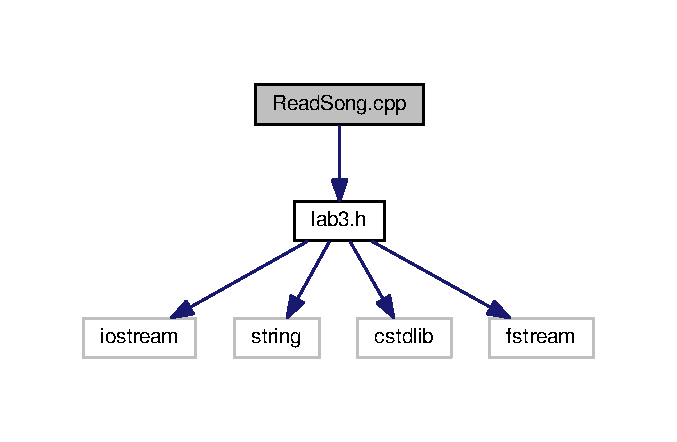
\includegraphics[width=325pt]{ReadSong_8cpp__incl}
\end{center}
\end{figure}
\subsubsection*{Functions}
\begin{DoxyCompactItemize}
\item 
void \hyperlink{ReadSong_8cpp_a465df42ae82d3c7db8516dc9d321450e}{read\+Song} (std\+::ifstream \&f, \hyperlink{structMUSICELMT}{M\+U\+S\+I\+C\+E\+L\+M\+T} music\mbox{[}$\,$\mbox{]}, int n)
\end{DoxyCompactItemize}


\subsubsection{Function Documentation}
\hypertarget{ReadSong_8cpp_a465df42ae82d3c7db8516dc9d321450e}{\index{Read\+Song.\+cpp@{Read\+Song.\+cpp}!read\+Song@{read\+Song}}
\index{read\+Song@{read\+Song}!Read\+Song.\+cpp@{Read\+Song.\+cpp}}
\paragraph[{read\+Song}]{\setlength{\rightskip}{0pt plus 5cm}void read\+Song (
\begin{DoxyParamCaption}
\item[{std\+::ifstream \&}]{f, }
\item[{{\bf M\+U\+S\+I\+C\+E\+L\+M\+T}}]{music\mbox{[}$\,$\mbox{]}, }
\item[{int}]{n}
\end{DoxyParamCaption}
)}}\label{ReadSong_8cpp_a465df42ae82d3c7db8516dc9d321450e}

\begin{DoxyCode}
5 \{
6     \textcolor{keywordtype}{int} i = 0; \textcolor{keywordtype}{char} type;
7     \textcolor{keywordflow}{while}(f >> type)
8     \{
9         \textcolor{comment}{//type = music[i].type;}
10         \textcolor{keywordflow}{if} (type == \textcolor{charliteral}{'n'})
11             \{
12             f >> music[i].\hyperlink{structMUSICELMT_a662fdb18330107012ed8902725b08e5c}{note}.\hyperlink{structNOTE_ae03dbb1306465fe61ec10da05fa5782e}{tone} >> music[i].\hyperlink{structMUSICELMT_a662fdb18330107012ed8902725b08e5c}{note}.\hyperlink{structNOTE_a258adf07267f95ab9630b33bad1b2fe2}{duration};
13             music[i].\hyperlink{structMUSICELMT_aa9a541d279b1a98b190c1968217ad37f}{type} = \hyperlink{lab3_8h_a41c816c739b4ab01c73879f01ae63880a3e1a299c993f58cef9ff1e4853051f02}{PLAYNOTE};
14             \}
15         \textcolor{keywordflow}{else} \textcolor{keywordflow}{if} (type == \textcolor{charliteral}{'f'})
16             \{
17             f >> music[i].\hyperlink{structMUSICELMT_ae418bce8087e7510ad8563a87b4c1c63}{fragment}.\hyperlink{structFRAGMENT_a9a2c77dc5f1c259a9a063f8e6ae18724}{start} >> music[i].\hyperlink{structMUSICELMT_ae418bce8087e7510ad8563a87b4c1c63}{fragment}.
      \hyperlink{structFRAGMENT_a3edee1f345e206cdc220b16d7d290018}{finish};
18             music[i].\hyperlink{structMUSICELMT_aa9a541d279b1a98b190c1968217ad37f}{type} = \hyperlink{lab3_8h_a41c816c739b4ab01c73879f01ae63880a0fab3b3b81cc5ad4ac6d6b74b50869e5}{PLAYFRAGMENT};
19             \}
20         i++;
21     \}
22     music[i].\hyperlink{structMUSICELMT_aa9a541d279b1a98b190c1968217ad37f}{type} = \hyperlink{lab3_8h_a41c816c739b4ab01c73879f01ae63880a2175f634cdffa7045d36d1b0cca00ed4}{PLAYSTOP};
23 \}
\end{DoxyCode}

\hypertarget{stack_8cpp}{\subsection{stack.\+cpp File Reference}
\label{stack_8cpp}\index{stack.\+cpp@{stack.\+cpp}}
}
{\ttfamily \#include \char`\"{}lab3.\+h\char`\"{}}\\*
Include dependency graph for stack.\+cpp\+:\nopagebreak
\begin{figure}[H]
\begin{center}
\leavevmode
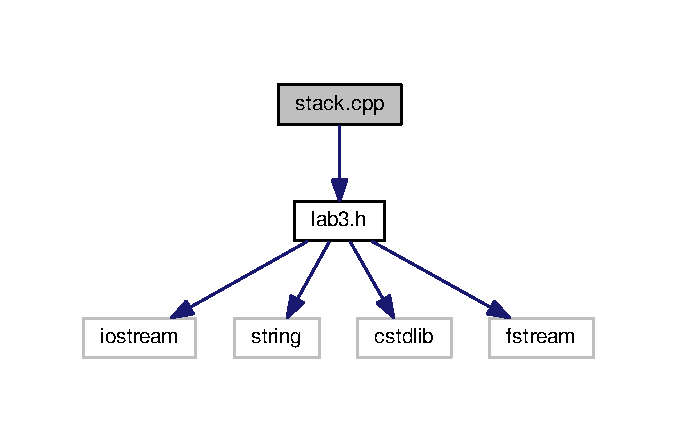
\includegraphics[width=325pt]{stack_8cpp__incl}
\end{center}
\end{figure}
\subsubsection*{Functions}
\begin{DoxyCompactItemize}
\item 
\hyperlink{lab3_8h_a32c27cc471df37f4fc818d65de0a56c4}{S\+T\+A\+T\+U\+S} \hyperlink{stack_8cpp_abd657d26045a775f57a837427142cfbd}{Create} (\hyperlink{structSTACK}{S\+T\+A\+C\+K} \&stack, int size)
\item 
\hyperlink{lab3_8h_a32c27cc471df37f4fc818d65de0a56c4}{S\+T\+A\+T\+U\+S} \hyperlink{stack_8cpp_a805a86f7ac8e643c87ea7d7cbb1b2c9c}{Push} (\hyperlink{structSTACK}{S\+T\+A\+C\+K} \&stack, int item)
\item 
\hyperlink{lab3_8h_a32c27cc471df37f4fc818d65de0a56c4}{S\+T\+A\+T\+U\+S} \hyperlink{stack_8cpp_a9ab82590ff3d7086853fd9b2106d255c}{Pop} (\hyperlink{structSTACK}{S\+T\+A\+C\+K} \&stack, int \&item)
\item 
void \hyperlink{stack_8cpp_a7f5d0e2c1d5c45b52ee6d1d91e420e95}{Destroy} (\hyperlink{structSTACK}{S\+T\+A\+C\+K} \&stack)
\end{DoxyCompactItemize}


\subsubsection{Function Documentation}
\hypertarget{stack_8cpp_abd657d26045a775f57a837427142cfbd}{\index{stack.\+cpp@{stack.\+cpp}!Create@{Create}}
\index{Create@{Create}!stack.\+cpp@{stack.\+cpp}}
\paragraph[{Create}]{\setlength{\rightskip}{0pt plus 5cm}{\bf S\+T\+A\+T\+U\+S} Create (
\begin{DoxyParamCaption}
\item[{{\bf S\+T\+A\+C\+K} \&}]{stack, }
\item[{int}]{size}
\end{DoxyParamCaption}
)}}\label{stack_8cpp_abd657d26045a775f57a837427142cfbd}

\begin{DoxyCode}
10 \{
11     stack.\hyperlink{structSTACK_a6d512f82cbd75729347a293193039538}{buf} = \textcolor{keyword}{new} \textcolor{keywordtype}{int}[size];
12     \textcolor{keywordflow}{if} (!stack.\hyperlink{structSTACK_a6d512f82cbd75729347a293193039538}{buf})
13         \textcolor{keywordflow}{return} \hyperlink{lab3_8h_a32c27cc471df37f4fc818d65de0a56c4aecedb56d1405a60c6069f4a0139bdec5}{FAILED};
14     stack.\hyperlink{structSTACK_ad10f9d8025122e8c82832d7a34c77e40}{size} = size;
15     stack.\hyperlink{structSTACK_a1b186cf876dace2f1e30fcbe260cad9a}{sp} = 0;
16     \textcolor{keywordflow}{return} \hyperlink{lab3_8h_a32c27cc471df37f4fc818d65de0a56c4a2bc49ec37d6a5715dd23e85f1ff5bb59}{OK};
17 \}
\end{DoxyCode}
\hypertarget{stack_8cpp_a7f5d0e2c1d5c45b52ee6d1d91e420e95}{\index{stack.\+cpp@{stack.\+cpp}!Destroy@{Destroy}}
\index{Destroy@{Destroy}!stack.\+cpp@{stack.\+cpp}}
\paragraph[{Destroy}]{\setlength{\rightskip}{0pt plus 5cm}void Destroy (
\begin{DoxyParamCaption}
\item[{{\bf S\+T\+A\+C\+K} \&}]{stack}
\end{DoxyParamCaption}
)}}\label{stack_8cpp_a7f5d0e2c1d5c45b52ee6d1d91e420e95}

\begin{DoxyCode}
44 \{
45     \textcolor{keyword}{delete} [] stack.\hyperlink{structSTACK_a6d512f82cbd75729347a293193039538}{buf};
46 \}
\end{DoxyCode}
\hypertarget{stack_8cpp_a9ab82590ff3d7086853fd9b2106d255c}{\index{stack.\+cpp@{stack.\+cpp}!Pop@{Pop}}
\index{Pop@{Pop}!stack.\+cpp@{stack.\+cpp}}
\paragraph[{Pop}]{\setlength{\rightskip}{0pt plus 5cm}{\bf S\+T\+A\+T\+U\+S} Pop (
\begin{DoxyParamCaption}
\item[{{\bf S\+T\+A\+C\+K} \&}]{stack, }
\item[{int \&}]{item}
\end{DoxyParamCaption}
)}}\label{stack_8cpp_a9ab82590ff3d7086853fd9b2106d255c}

\begin{DoxyCode}
33 \{
34     
35     \textcolor{keywordflow}{if} (stack.\hyperlink{structSTACK_a1b186cf876dace2f1e30fcbe260cad9a}{sp} == 0)
36         \textcolor{keywordflow}{return} \hyperlink{lab3_8h_a32c27cc471df37f4fc818d65de0a56c4aecedb56d1405a60c6069f4a0139bdec5}{FAILED};
37     stack.\hyperlink{structSTACK_a1b186cf876dace2f1e30fcbe260cad9a}{sp}--;
38     item = stack.\hyperlink{structSTACK_a6d512f82cbd75729347a293193039538}{buf}[stack.\hyperlink{structSTACK_a1b186cf876dace2f1e30fcbe260cad9a}{sp}];
39     \textcolor{keywordflow}{return} \hyperlink{lab3_8h_a32c27cc471df37f4fc818d65de0a56c4a2bc49ec37d6a5715dd23e85f1ff5bb59}{OK};
40 
41 \}
\end{DoxyCode}
\hypertarget{stack_8cpp_a805a86f7ac8e643c87ea7d7cbb1b2c9c}{\index{stack.\+cpp@{stack.\+cpp}!Push@{Push}}
\index{Push@{Push}!stack.\+cpp@{stack.\+cpp}}
\paragraph[{Push}]{\setlength{\rightskip}{0pt plus 5cm}{\bf S\+T\+A\+T\+U\+S} Push (
\begin{DoxyParamCaption}
\item[{{\bf S\+T\+A\+C\+K} \&}]{stack, }
\item[{int}]{item}
\end{DoxyParamCaption}
)}}\label{stack_8cpp_a805a86f7ac8e643c87ea7d7cbb1b2c9c}

\begin{DoxyCode}
23 \{
24 
25     \textcolor{keywordflow}{if} (stack.\hyperlink{structSTACK_a1b186cf876dace2f1e30fcbe260cad9a}{sp} == stack.\hyperlink{structSTACK_ad10f9d8025122e8c82832d7a34c77e40}{size})
26         \textcolor{keywordflow}{return} \hyperlink{lab3_8h_a32c27cc471df37f4fc818d65de0a56c4aecedb56d1405a60c6069f4a0139bdec5}{FAILED};
27     stack.\hyperlink{structSTACK_a6d512f82cbd75729347a293193039538}{buf}[stack.\hyperlink{structSTACK_a1b186cf876dace2f1e30fcbe260cad9a}{sp}] = item;
28     stack.\hyperlink{structSTACK_a1b186cf876dace2f1e30fcbe260cad9a}{sp}++;
29     \textcolor{keywordflow}{return} \hyperlink{lab3_8h_a32c27cc471df37f4fc818d65de0a56c4a2bc49ec37d6a5715dd23e85f1ff5bb59}{OK};
30 \}
\end{DoxyCode}

%--- End generated contents ---

% Index
\newpage
\phantomsection
\addcontentsline{toc}{section}{Index}
\printindex

\end{document}
